\documentclass{article}
\usepackage{listings}
\usepackage[utf8]{inputenc}
\usepackage{graphicx}
\renewcommand{\figurename}{Figura}
\usepackage{mathtools}

\title{Informe de Estadística en Física Experimental: Ejercicio 15 Guía 2}
\author{Andr\'es Babino}

\begin{document}
\maketitle

\section{Item a}
Abajo copio el código de un programa que cuenta el número de éxitos de n experimentos de bernulli  con probabilidad de éxito p.
\begin{lstlisting}
def binomial_sample(n, p):
    """
    Take a sample of size n from a binomial distribution with
    success probability equal p.
    Returns the number of sucesses.
    """
    s = 0
    for i in xrange(n):
        x = random.random()
        if x < p:
            s += 1
    return s
\end{lstlisting}
El código está implementado en python y usa el paquete estandar \textit{random}.

\section{Item b}
En la figura \ref{fig:itemb} se muestra un histograma que se obtiene utilizando la función anterior 1000 veces.
El parámetro p se tomó igual a 0.7 y el parámetro n igual a 15.
Estos parámetros simulan un experimento hipotético en el que mil veces 15 fotones impactan un detector con una eficiencia del 70\%.
En negro se graficó la distribución de probabilidad de binomial $B(1000, 0.7)$.

\begin{figure}
\centering
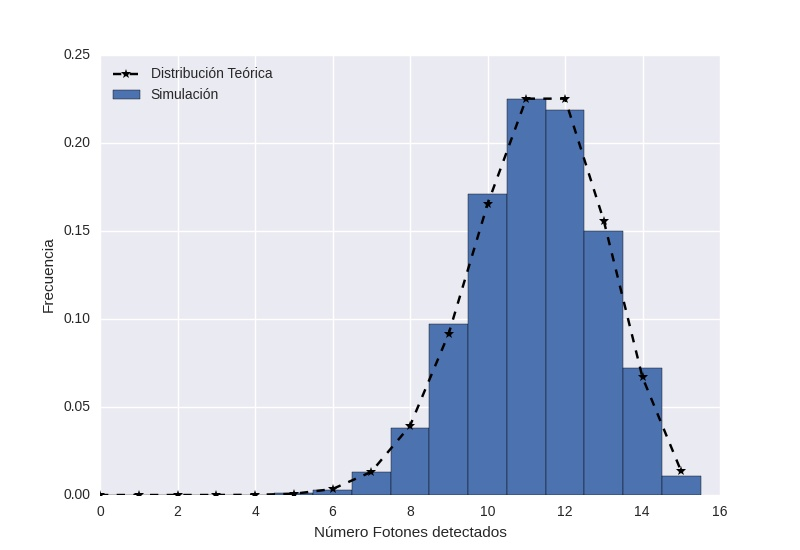
\includegraphics[width=0.75\textwidth]{figb.jpg}
\caption[]{Histograma del item b}
\label{fig:itemb}
\end{figure}

\section{Item c}
Ahora consideremos una funete de intensidad media $I=15\ fot\ s^{-1}$.
La distribución de fotones emitidos en un intervalo de tiempo $t$ seguirá una ditribuión de Poisson.

$$\text{número\ de\ fotones} = \frac{(\lambda t)^k}{k!} e^{-\lambda t}$$

En la figura \ref{fig:poisson} vemos la distribución de Poisson cuando $\lambda=15$ y $t=0.001$.
Con estos parámetros la probabilidad de que no ocurra ningún evento es del 98.51\% y la probabilidad de que ocurra un único evento es del $1.48\%$.
Estas dos probabilidades sumadas dan $99.99\%$  lo que quiere decir que la probabilidad de que sucedan dos o más eventos es $0.01\%$.
Vemos que la probabilidad de que ocurran 2 eventos es suficientemente pequeña como para suponer que no se observaran este tipo de eventos si repetimos el experimento $1000$ veces, es decir durante $1s$.
Es por esto que podemos simular la emisión de fotones como una sucesión de eventos binomiales.

\begin{figure}
\centering
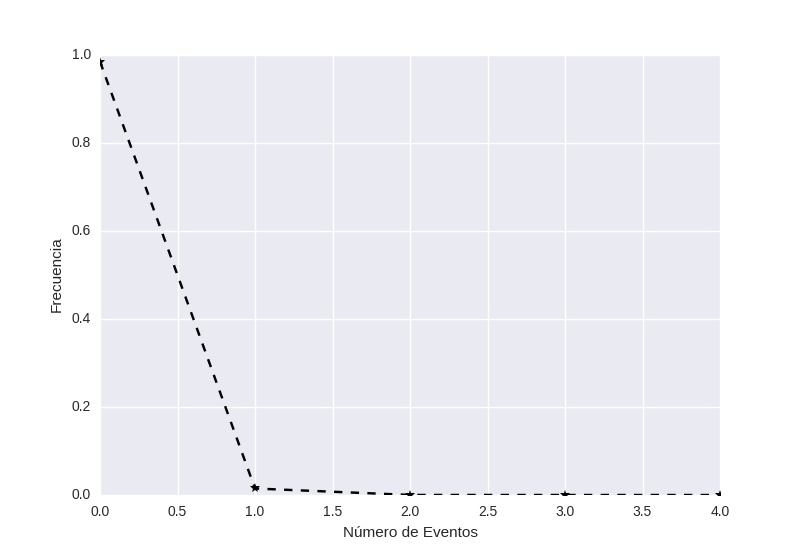
\includegraphics[width=0.75\textwidth]{poisson.jpg}
\caption[]{Distribución de probabilidad de Poisson con paramtetro $\lambda=0.015$}
\label{fig:poisson}
\end{figure}

Con esto en mente utilizamos nuevamente el programa \textit{binomial\_sample} para simular una fuente con estas características.
En la figura \ref{fig:itemc} se observa el histograma de eventos simulados de esta manera y en linea negra la distribución de Poisson correspondiente. Se observa un buen acuerdo, lo que significa que la aproximación que hicimos es razonable.

\begin{figure}
\centering
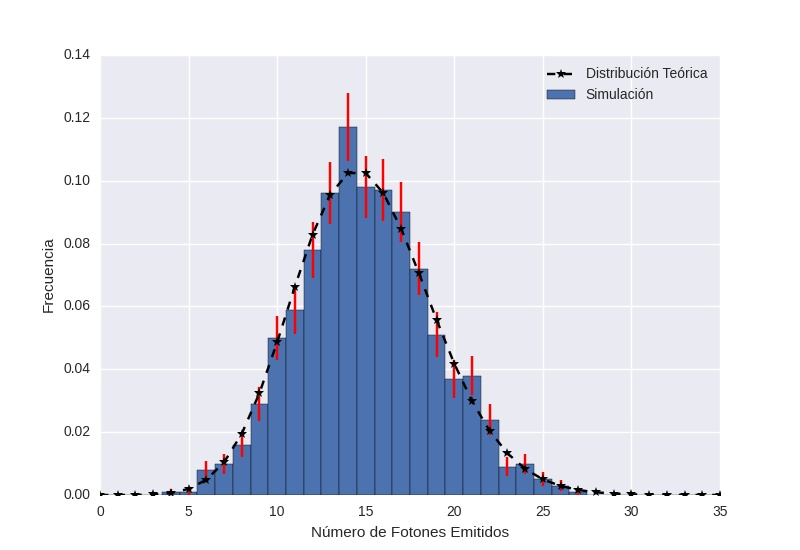
\includegraphics[width=0.75\textwidth]{figc.jpg}
\caption[]{Histograma del item c}
\label{fig:itemc}
\end{figure}

\section{Item d}
Ahora vamos a utilizar cada uno de los 1000 ensayos de emisión de fotones simulados en el ítem c como entrada para el detector simulado en el ítem b b.
Lo que obtenemos es una simulación del número de fotones detectados por el detector que fueron emitidos por la fuente.
El histograma de esta simulación se puede ver en la figura  \ref{fig:itemd}.

La producción de fotones en la fuente sigue una distribución de Poisson y el número de fotones detectados dado el arrivo de n fotones sigue una distribución binomial.
Ahora nos preguntamos cúal será la distribución de fotones detectados dado el arrivo de los fotones producidos con una distribución de Poisson.
La probabilidad de que se detecten k fotones será:
$$
P(k) = \sum_{k=n}^{\infty} B_k(n, \epsilon) P_n(\lambda t)
$$
donde $B_k(n, \epsilon)$ es la distribución binomial que describe el proceso de medición y $P_n(\lambda t)$ es una distribución de Poisson que describe el proceso de producción de fotones.
Si escribimos la definición de estas distribuciones obtenemos:
$$
P(k) = \sum_{k=n}^{\infty} \frac{n!}{k!(n-k)!}\epsilon^k (1- \epsilon)^(n-k) \frac{(\lambda t)^n}{n!}e^{-\lambda t}
$$

Definiendo $m=n-k$ y sacando todo lo que no depende de $m$ fuera de la suma obtenemos:

$$
P(k) = \frac{\epsilon^k (\lambda t)^k e^{-\lambda t}}{k!} \sum_{m=0}^{\infty} \frac{[\lambda t(1- \epsilon)]^m}{m!}
$$

Escrito así el sumando es la definición de la exponencial $e^{\lambda t(1- \epsilon)}$.
Agrupando obtenemos:

$$
P(k) = \frac{(\epsilon \lambda t)^k}{k!} e^{-\epsilon \lambda t}
$$

Que es una distribución de Poisson con constanle $\epsilon \lambda t$.
Por lo tanto para comparar nuestro histograma de la figura \ref{fig:figd} debemos usar una distribución de Poisson con constante $10.5$.
En la figura \ref{fig:figd} se ve en negro esta distribución y se observa que se corresponde con los datos simulados.


\begin{figure}
\centering
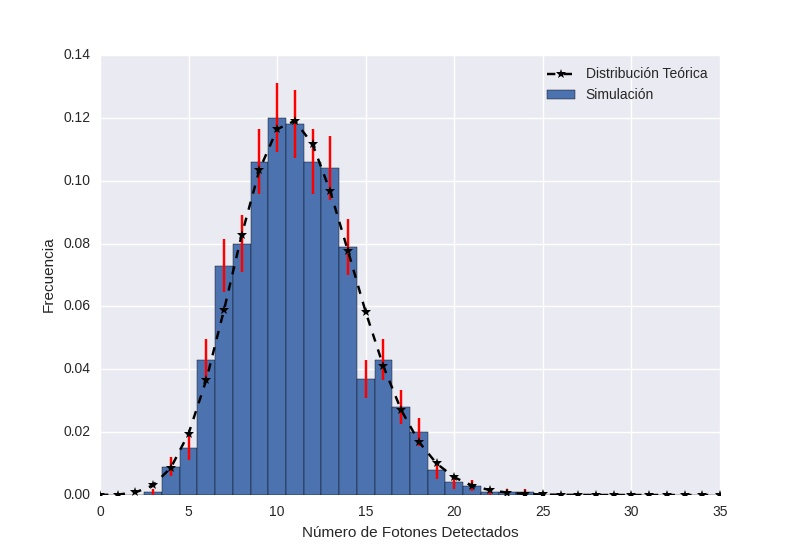
\includegraphics[width=0.75\textwidth]{figd.jpg}
\caption[]{Histograma del item d}
\label{fig:itemd}
\end{figure}

\section{Item e}
\begin{figure}
\centering
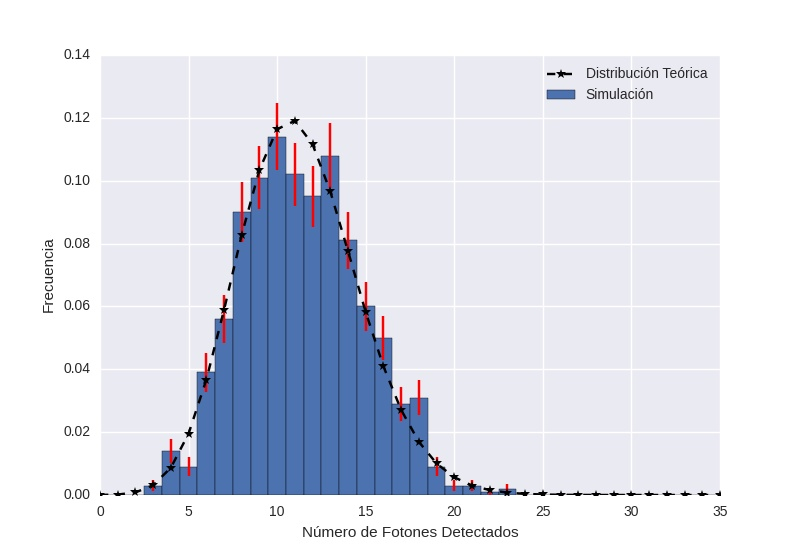
\includegraphics[width=0.75\textwidth]{fige.jpg}
\caption[]{Histograma del item e}
\label{fig:iteme}
\end{figure}

\section{Item f}
\end{document}
